\documentclass[letter]{article}
\usepackage[margin=1in]{geometry}
%\documentclass[10pt]{article}
\usepackage[final]{graphicx}
\usepackage{color}


%\usepackage[cm]{fullpage}
\usepackage{
amsfonts,amssymb,
amsmath,
url,graphics,subfig,
cite,
calc,
psfrag, bm,
amsthm, 
paralist}

%\renewcommand{\textwidth}{5.5in}

%---- Some math. macro
\newcommand\infsum[1][n]{\ensuremath{\sum_{#1=-\infty}^\infty}}

% Here's the definition of Sb, stolen from amstex
    \makeatletter
    \def\multilimits@{\bgroup
  \Let@
  \restore@math@cr
  \default@tag
 \baselineskip\fontdimen10 \scriptfont\tw@
 \advance\baselineskip\fontdimen12 \scriptfont\tw@
 \lineskip\thr@@\fontdimen8 \scriptfont\thr@@
 \lineskiplimit\lineskip
 \vbox\bgroup\ialign\bgroup\hfil$\m@th\scriptstyle{##}$\hfil\crcr}
    \def\Sb{_\multilimits@}
    \def\endSb{\crcr\egroup\egroup\egroup}
\makeatother

\newtheoremstyle{t}         %name
    {\baselineskip}{2\topsep}      %space above and below
    {\rm}                   %Body font
    {0pt}{\bfseries}  %Heading indent and font
    {~}                      %after heading
    { }                      %head after space
    {\thmname{#1}\thmnumber{#2}.}

%\theoremstyle{t}
%\newtheorem{q}{Q}
\parindent=0pt 

\newtheorem{Lemma}{Lemma}
\newtheorem{prop}{Proposition}
\newtheorem{Theorem}{Theorem}
\newtheorem{Corollary}{Corollary}
\newtheorem{Claim}{Claim}
\newtheorem{Fact}{Fact}
\newtheorem{Observation}{Observation}


\theoremstyle{remark}
\newtheorem{Remark}{Remark}
\newtheorem{Example}{Example}


\begin{document}

\setcounter{page}{1}
\linespread{1.1}
\normalsize

\setlength{\parskip}{.2cm}

\begin{center} {\Large \textbf{
ECS289F Progress report\vspace{.2cm} \\ --- Opinion Dynamics with  reluctant agents ---}} \vspace{.3cm}

{Hoi-To Wai, Christopher Patton}

\today

\end{center}
\vspace{0.1cm}


% \begin{abstract}
%This note is a summary of the rudimentary ideas I have for ECS289F's project. Specifically, I will propose a model for the opinion dynamics with reluctant agents, i.e., agents who are reluctant to blend their idea with his/her neighbors. Explorations into the Bitcoin attack model will also be investigated. (For the references cited here, I believe that better references must exists, but I will need to spend more time on mining them.)
%\end{abstract}


%-----------------------------------------------------------------------------
%\vspace{0.5cm}

%\section{Introduction} \vspace{-.3cm}
This document reports on the recent progress we have made for the course project in the two weeks after the project proposal's submission. The goal of this project is to consider a new aspect for the DeGroot's model by considering an opinion dynamic model where a subset of agents are \emph{reluctant} to update their opinion. 

%The idea of modeling opinion dynamics has been pioneered by DeGroot \cite{Degroot_74}. He proposes a simple model of social interactions in which both the time it will take to reach consensus, as well as the consensus score itslf, can be computed easily. Though this model has proven to be insightful in this domain, it doesn't capture the dynamics of many consensus scenarios. Namely, we would like to capture the throughput and latency dynamics of censor networks. 

Let us first recap on the system model.
We consider an undirected graph $G = (V,E)$ with $|V| = n$. Each agent $i \in V$ holds an initial opinion ${\bm w}_i^{(0)} \in \mathbb{R}^L$. At time $k$, the agents exchange their beliefs with the others to compute:
\begin{equation}\label{eq:op}
\hat{\bm w}_i^{(k)} = \sum_{j \in \mathcal{N}_i} A_{ij}^{(k)} {\bm w}_j^{(k-1)},
\end{equation}
where $0 \leq A_{ij}^{(k)} \leq 1$ models the trust agent $i$ has on agent $j$ at time $k$. Importantly, we assume $\sum_{j=1}^{|V|} A_{ij}^{(k)} = 1$ and $\sum_{i=1}^{|V|} A_{ij}^{(k)} = 1$. Notice that the matrix ${\bm A}^{(k)}$ is time-variant and it is randomly generated at each $k$. 

In the subsequent analysis, we shall focus on the so-called \emph{randomized gossip model} \cite{}. The mixing matrix ${\bm A}^{(k)}$ is given as:
\[
{\bm A}^{(k)} = {\bf I} - \frac{1}{2} ({\bf e}_i + {\bf e}_j) ({\bf e}_i + {\bf e}_j)^T,
\]
where $(i,j) \in E$ is an edge of $E$ selected uniformly and independently at time $k$. The model represents the scenario when agents communicate by `gossiping', i.e., at each time there can only be two agents exchanging idea with each other. 


The vector $\hat{\bm w}_i^{(k)}$ is the opinion that agent $i$ is supposed to hold at time $k$. In DeGroot's model, the agents are updating instantly such that ${\bm w}_i^{(k)} = \hat{\bm w}_i^{(k)} $. In this case, it is known that ${\bm w}_i^{(k)}$ converges to the average of $\{{\bm w}_i^{(0)} \}$ asymptotically, i.e., achieving the `wisdom of the crowd',  under some mild assumptions. 
For instance, the result can be easily obtained by exploiting the property that the sequence of random matrice $\{ {\bm A}^{(k)} \}$ is an independent process. 

In this project, we consider a new type of agent called the `reluctant' agent. Upon exchanging their beliefs with their neighbors, they don't update \emph{immediately}. Instead, ${\bm w}_i^{(k)}$ is updated by:
\begin{equation} \label{eq:adapt}
{\bm w}_i^{(k)} = \frac{\min\{ c_i^{(k)}, \tau_i\} }{\tau_i} \hat{\bm w}_i^{(k - c_i^{(k)} + 1)} + \frac{\tau_i - \min\{ c_i^{(k)}, \tau_i\} }{\tau_i} {\bm w}_i^{(k-c_i^{(k)})},~i \in V_r,
\end{equation}
where $V_r \subseteq V$ is the set of reluctant agents, $c_i^{(k)}$ is a counter variable such that
\[
c_i^{(k)} = \begin{cases}
1 &,~{\rm if}~A_{ij}^{(k)} \neq 0,~\text{for some}~j \in V~\text{(agent $i$ talked at time $k$)}. \\
c_i^{(k-1)} + 1 &,~{\rm otherwise}
\end{cases}
\]
and $\tau_i \in \mathbb{Z}$ is the adaptation rate of $i$. From \eqref{eq:adapt}, it is important to clarify the mechanism that reluctant agent updates: i) the reluctant agent will slowly adapt to the new opinion in $\tau_i$ time steps; ii) if the agent is `interrupted' during the adaptation process, it will \emph{restart} the adaptation process based on ${\bm w}_i^{(k-1)}$. This is similar to having a reluctant agent that is greedy/eager to switch his/her belief.

We shall discuss the motivation and possible extensions/applications of the above model towards the end of this report.

%\subsection{Project goal and deliverables} 

\subsection{Previous works and references} 
Our work is based upon the pioneering paper by DeGroot \cite{Degroot_74} and a recent survey in \cite{Fagnani2014}. Furthermore, the reluctant agent model is inspired by \cite{Acemoglu2013}, which has studied the effect of \emph{stubborn} agents in a social network. For the simulation, we may also follow the reference \cite{Das2014} which has conducted experiments on opinion dynamics using real data. 

While we are conducting the convergence analysis, we found that the references \cite{Nedic2010} have provided a nice framework for us to develop our theories. In particular \cite{Nedic2010} has considered and analyzed a delayed consensus model. In addition, the recent result from \cite{Touri2014} will also be applied in the analysis. 


%For the convergence analysis, 


\section{Convergence Analysis} 
In this section, we perform a convergence analysis for the proposed opinion dynamics model using randomized gossip exchange. 
The main result (so far) is that we can establish that the opinions will  converge to a (biased) consensus almost surely. 
As a preliminary observation, we found that the converged opinion will be biased towards the initial opinions of the reluctant agent in expectation. 

%We propose to analyze our model under the framework of \cite{}. The latter reference has studied a delayed consensus model by considering an augmented system with a few extra nodes that models the delay in the system. The augmented system is delay-free and it can subsequently be analyzed. 
Our analysis is inspired by \cite{Nedic2010} and applies the result in \cite{Touri2014}. Specifically, we introduce the augmented nodes such that the reluctant opinion dynamics model can be recast into the simple form of 
\[
\tilde{\bm w}_i^{(k)} = \sum_{j=1}^{|V'|} \bar{A}_{ij}^{(k)} \tilde{\bm w}_j^{(k-1)}
\]
To this end, let us consider a directed graph $G' = (V',E')$ where $V'$ contains all the nodes from $V$ together with a few augmented node, defined as follows. For each $i \in V_r$, we define $2$ new nodes denoted by $\{ i', i'' \}$. Here, the $i'$th node stores the value of $\hat{\bm w}_i^{(k)}$ and the $i''$th node stores the value of old ${\bm w}_i^{(k)}$. The inter-connectivity of these nodes are best illustrated by the example in Fig.~\ref{fig:augment}. 

\begin{figure}[t]
\centerline{\resizebox{.5\textwidth}{!}{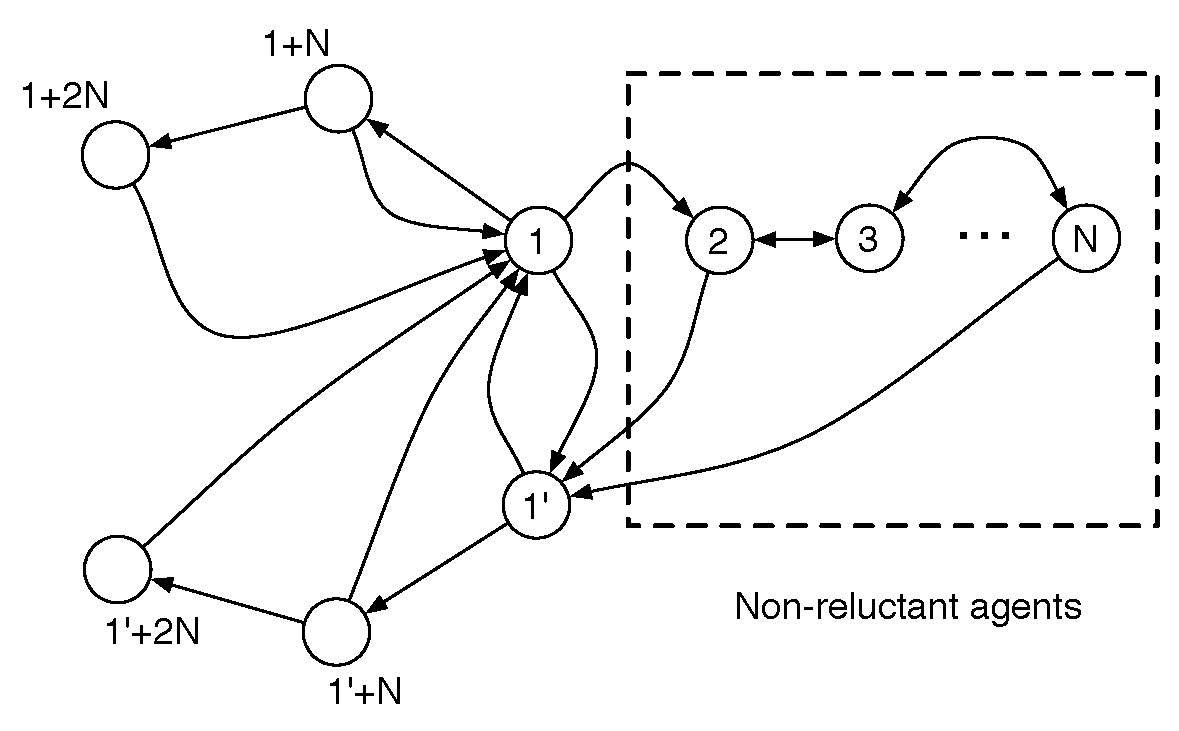
\includegraphics{./augmented_graph}}
}
\caption{Example of the augmented system for $V_r = \{1\}$. 
} \label{fig:augment}
\end{figure}

Using the augmented system $G'$, we can describe the equivalent opinion dynamics that executes on the graph. In particular, we split the update dynamics at time $k$ to two steps $k$ and $k'$. Step $k$ corresponds to the update stage \eqref{eq:op} and step $k'$ corresponds to the adaptation stage \eqref{eq:adapt}. 
Additionally, the counter variable $c_i^{(k)}$ is defined as before and they are updated before step $k$. 

Let $\tilde{ \bm w}_i$ be the opinion held by agent $i$ in the augmented system, the system is initialized as follows.
\[
c_i^{(0)} = M,~\forall~ i \in V'~{\rm and}~\tilde{ \bm w}_i^{(0)} = \begin{cases} { \bm w}_i^{(0)} &,~i \in V \\
 {\bf 0} &,~i \in V' \setminus V, \end{cases}
\]
where $M > \tau_i$ for all $i$ enforces a `reset' state for the adaptation process. 

\textbf{Updating stage}: At the \emph{updating} stage, we have that 
\[
\tilde{\bm w}_i^{(k)} = \sum_{j \in \mathcal{N}_i} A_{ij}^{(k)} \tilde{\bm w}_j^{(k-1)'},~i \in V \setminus V_r,
\]
i.e., the non-reluctant agents are updated immediately. 
As for node $i \in V_r$, we have $$\tilde{\bm w}_i^{(k)} = \tilde{\bm w}_i^{(k-1)'}$$ such that it is left intact. 
For node $i'$ where $i \in V_r$, we have:
\[
\tilde{\bm w}_{i'}^{(k)} = \begin{cases}
\displaystyle \sum_{j \in \mathcal{N}_i} A_{ij}^{(k)} \tilde{\bm w}_j^{(k-1)'}&,~{\rm if}~c_i^{(k)} = 1. \\
\tilde{\bm w}_{i'}^{(k-1)'}&,~{\rm otherwise},
\end{cases}
\]
and for node $i''$ where $i \in V_r$, 
\[
\tilde{\bm w}_{i''}^{(k)} = \begin{cases}
\tilde{\bm w}_{i}^{(k-1)'}&,~{\rm if}~c_i^{(k)} = 1. \\
\tilde{\bm w}_{i''}^{(k-1)'}&,~{\rm otherwise}.
\end{cases}
\]
The two equations above describes the opinion dynamics that when the counter variable $c_i^{(k)}$ is reset, then the stored variables will be updated. 

Let us define $\tilde{\bm A}^{(k)}$ as the overall updating matrix in this stage, i.e., we have:
\[
\tilde{\bm w}_i^{(k)} = \sum_{j=1}^{|V'|} \tilde{A}_{ij}^{(k)} \tilde{\bm w}_j^{(k-1)'}.
\]
It can be verified that $\tilde{\bm A}^{(k)}$ is stochastic. 

%Moreover, the updated opinion will be stored in the $i'$th node if $i$ is a reluctant agent:
%\[
%\tilde{\bm w}_{i'}^{(k)} = \sum_{j \in \mathcal{N}_i} A_{ij}^{(k)} \tilde{\bm w}_j^{(k-1)'},~i \in  V_r,
%\]
%The opinions at the other augmented nodes are updated as follows:
%\[
%\tilde{\bm w}_{i+j N}^{(k)} = \tilde{\bm w}_{i + (j-1)N}^{(k-1)'},~j=1,...,\tau_i - 1,~i \in V_r,
%\]
%\[
%\tilde{\bm w}_{i' +j N}^{(k)} = \tilde{\bm w}_{i' + (j-1)N}^{(k-1)'},~j=1,...,\tau_i - 1,~i \in V_r.
%\]
%To summarize, let us define $\tilde{\bm A}^{(k)}$ as the updating matrix in this stage, we have:
%\[
%\tilde{\bm w}_i^{(k)} = \sum_{j=1}^{|V'|} \tilde{A}_{ij}^{(k)} \tilde{\bm w}_j^{(k-1)'}
%\]
%where $\tilde{\bm A}^{(k)}$ is:
%\begin{equation} \label{eq:a_update}
%\tilde{A}_{ij}^{(k)} = \begin{cases}
%A_{ij}^{(k)} &,~i \in V \setminus V_r, \\
%A_{ij}^{(k)} &,~i = i', \\
%1 &,~i = j~{\rm and}~i \in V_r,\\
%1 &,~i = m + \ell N,~j=m + (\ell-1) N~{\rm for~some}~m \in V_r, \\
%1 &,~i = m' + \ell N,~j=m' + (\ell-1) N~{\rm for~some}~m \in V_r, \\
%0 &,~{\rm otherwise}.
%\end{cases}
%\end{equation}

\textbf{Adaptation stage}: At the \emph{adaptation} stage, the non-reluctant agents and the augmented nodes will remain unchanged, i.e.,
\[
\tilde{\bm w}_i^{(k')} = \tilde{\bm w}_i^{(k)},~i \in V' \setminus V_r.
\]
However, the opinion of the reluctant agent will be adapted using the stored information in node $i'$ and $i''$:
\[
\tilde{\bm w}_i^{(k')} = \begin{cases}
\displaystyle \frac{c_i^{(k)}}{\tau_i} \tilde{\bm w}_{i'}^{(k)} + \frac{\tau_i - c_i^{(k)}}{\tau_i} \tilde{\bm w}_{i''}^{(k)} &,~{\rm if}~c_i^{(k)} \leq \tau_i, \vspace{.2cm} \\
\tilde{\bm w}_i^{(k)} &,~{\rm otherwise}.
\end{cases}
\]
With some efforts, the dynamics described above can also be written using an update matrix $\tilde{\bm A}^{(k')}$. Such $\tilde{\bm A}^{(k')}$ is also found to be stochastic.

To summarize, we can now write the opinion dynamics as:
\[
\tilde{\bm w}_i^{(k')} = \sum_{j=1}^{|V'|} \tilde{A}_{ij}^{(k')} \sum_{\ell=1}^{|V'|} \tilde{A}_{j \ell}^{(k)} \tilde{\bm w}_{\ell}^{(k-1)'} =  \sum_{j=1}^{|V'|} \bar{A}_{ij}^{(k)} \tilde{\bm w}_{j}^{(k-1)'},
\]
where $\bar{\bm A}^{(k)} = \tilde{\bm A}^{(k')}  \tilde{\bm A}^{(k)}$ is a stochastic matrix for all $k$. 

%We are interested in . 
%It turns out that the result is not trivial to obtain. 
We now analyze the convergence properties of the above model.
The main challenge is that the update matrix $\bar{\bm A}^{(k)}$ is correlated with its previous realizations, e.g., $\bar{\bm A}^{(k-1)}, ..., \bar{\bm A}^{(1)}$. 
However, using a recent result from \cite{Touri2014}, we are able to prove the following. 
%To prove the main result of the convergence analysis, we apply a recent result from \cite{}. 

Let us define 
\[
\bm{\Phi} (s+t,s) = \bar{\bm A}^{(s+t)}  \bar{\bm A}^{(s+t-1)} \ldots  \bar{\bm A}^{(s)}
\]
The result from \cite{Touri2014} requires the so-called \emph{balancedness} property. The latter property can be shown as a consequence of the claim that there exists $\eta, t > 0$ with:
\begin{equation} \label{eq:claim}
E \left( [\Phi (k+t,k)]_{ij} | \mathcal{F}_{k} \right) \geq \eta E \left( [\Phi (k+t,k)]_{ji} | \mathcal{F}_{k} \right),~\forall~i,j,k,
\end{equation}
where $ \mathcal{F}_{k}  = \{  \bar{\bm A}^{(k-1)},  \bar{\bm A}^{(k-2)}, ...,  \bar{\bm A}^{(1)} \}$ denotes the events that happened in the past (prior to the $k$th time step). 
%As coined in \cite{}, the opinion dynamics of our model is called a \emph{balanced} process
%The result can be applied as follows. 

A rigorous proof for this claim is more technical and will not be pursued here. However, to gain some insights, if we assume that the original graph $G$ is fully connected, then \eqref{eq:claim} can be satisfied for $t = 2$. The reason is that there is a non-zero probability for any two nodes  in the augmented system to communicate with each other in 2 hops. 

As a consequence of the claim and \cite{Touri2014}, we have:
\begin{prop}
As the reluctant update model constitutes a balanced process, the opinions in reluctant updates model reach consensus almost surely, i.e., we have
% in the expectation as $k \rightarrow \infty$. We have
\begin{equation} \label{eq:propo}
\lim_{k \rightarrow \infty} P \left( \prod_{\ell=1}^{k} \bar{\bm A}^{(\ell)} = {\bf 1} ({\bm \pi}^\star)^T \right) = 1,
\end{equation}
for some ${\bm \pi}^\star \in \mathbb{R}^{|V'|}$ and ${\bf 1}^T {\bm \pi}^\star = 1$.
\end{prop}

The proof for Proposition~1 is skipped as it is a direct application of \cite{Touri2014}.
%{\color{red} I haven't looked into the proof of the theorem in \cite{} yet.} 
Proposition~1 implies that the dynamic model with the reluctant agents still reaches a consensus asymptotically. However, it is likely that the consensus reached will be biased, i.e., it differs from the true average. Notice that this happens when ${\bm \pi}^\star \neq {\bf 1} / |V'|$. In the subsequent analysis, we shall evaluate the magnitude of such bias empirically. 

%To obtain the desired result, we observe  that if ${\bm A}^{(k)}$ is stochastic, then $\tilde{\bm A}^{(k)}$ is also stochastic. To summarize, we have:
%\begin{prop}
%%Assuming that $\{ {\bm A}^{(k)} \}$ constitutes a sequence of opinion updates that lead to  consensus in the DeGroot's model as $k \rightarrow \infty$, then 
%The opinions in reluctant updates model reach consensus in the expectation as $k \rightarrow \infty$. We have
%\[
%\lim_{k \rightarrow \infty} E \left\{ \prod_{\ell=1}^{k} \tilde{\bm A}^{(\ell')} \tilde{\bm A}^{(\ell)} \right\} = {\bf 1} ({\bm \pi}^\star)^T,
%\]
%for some ${\bm \pi}^\star \in \mathbb{R}^{|V'|}$.
%\end{prop}

\subsection{Insights from the analysis using numerical simulations}
We are interested in estimating the value of $E [ \bm{\pi}^\star ]$ in \eqref{eq:propo}. As mentioned before, evaluating the expected value analytically is non-trivial as the chain $\{ \bar{\bm A}^{(k)} \}$ is not independent. Here, we perform numerical simulations to estimate $E [ \bm{\pi}^\star ]$. As we shall see later, this analysis shows that the system will tend to bias towards the (initial) opinions of the reluctant agents. 

As a preliminary study, we consider a fully connected network with $N=10$ agents. There are $|V_r| = 2$ reluctant agents which are the first two agents in the system. Moreover, we have $\tau_1 = \tau_2 = 20$. Through modeling the network as the augmented system, we find that the corresponding $E[\bm{\pi}^\star]$ (by averaging over 1000 Monte-Carlo trials) is 
\[
E[\bm{\pi}^\star] = \left[  {\bf 0.2560~0.2521}~0.0616~ 0.0613~0.0607~0.0619~0.0610~ 0.0606~0.0626~0.0621~0~0~0~0 \right],
\]
where the last 4 entries corresponds to the augmented nodes. Moreover, if $\tau_1 = \tau_2 = 2$, we have:
\[
E[\bm{\pi}^\star] = \left[  {\bf 0.1095~0.1081}~0.0978~0.0975~0.0980~0.0980~0.0980~0.0978~0.0978~0.0976~0~0~0~0 \right].
\]

There are two observations we can draw from the above analysis. Firstly, instead of converging to an all-one vector, $E[\bm{\pi}^\star]$ has  a heavier weight on the reluctant agents. This confirms that there is a bias associated with the network composed of reluctant agents. Secondly, the more \emph{reluctant} the agents are, the more bias will be resulted. This is a reasonable result as the reluctant agents have higher chance to influence the others simply due to the fact that they are reluctant. 

The above observation also leads to a \emph{bias-equalization} approach that tries to cancel the bias induced by the reluctant agent. In particular, we may initialize ${\bm w}_i^{(0)}$ by:
\[
({\bm w}_i^{(0)})' = \frac{{\bm w}_i^{(0)}}{ (E[\bm{\pi}^\star])_i }
\]
However, such an approach may not work if we also look at the second order statistics of $\bm{\pi}^\star$. That is, we evaluate $\sigma_i = \sqrt{E[ (\pi_i - E[\pi_i])^2 ]}$. For $\tau_1 = \tau_2 = 20$, we have
\[
\bm{\sigma} = \left[  {\bf 0.0566~0.0535} ~0.0186~0.0167~0.0176~0.0184~0.0175~0.0163~0.0172~0.0181~0~0~0~0 \right],
\]
and for $\tau_1 = \tau_2 = 2$, we get
\[
\bm{\sigma} = \left[  {\bf 0.0137~0.0146} ~0.0075~0.0079~0.0078~0.0078~0.0074~0.0079~0.0078~0.0076~0~0~0~0 \right],
\]
In both cases, we observe that the standard deviation of $\bm{\pi}^\star$ is rather high. 

%To summarize, we believe that the results above are reasonable as the reluctant agents have higher chance to influence the others. One may 

\section{Simulation Studies}

\section{Extensions and applications of the model}


%We will study how the reluctant agent will affect the consensus result in the model. In the first stage, we will examine (via simulation) the bias introduced by adding reluctant agents. How do topological properties, such as degree distribution, betweenness, and centrality impact the bias? and what about the speed of convergence? These questions will be addressed both analytically and empirically with respect to a few rew relevant network models discussed in class. A concrete result of this work will be a suite of tools for simulating various consensus scenarious on hand of real as well as synthetic data. 
%
%As an extension, we will study if we can recover the `wisdom of the crowd' given that we know some agents are reluctant. Another possible extension will be to consider discrete opinion dynamics. \vspace{-.2cm}
%



%\renewcommand{\refname}{\vspace{-1.5cm}}
%\small
\bibliographystyle{IEEEtran}
\bibliography{paper}


\end{document}
